\section{LLVM}

It is worth mentioning that there exist many compiler-specific preprocessor directives.
For portability reasons it is encouraged to avoid using them, though there is one
exception to this rule\footnote{Further reading: \url{https://en.wikipedia.org/wiki/Pragma_once}.}
(\path{#pragma once}). In general, a compiler is best thought of as a collection
of seven sequential phases, though in reality their implementation is more intertwined
than distinct from each other.

\begin{figure}[ht]
    \centering
    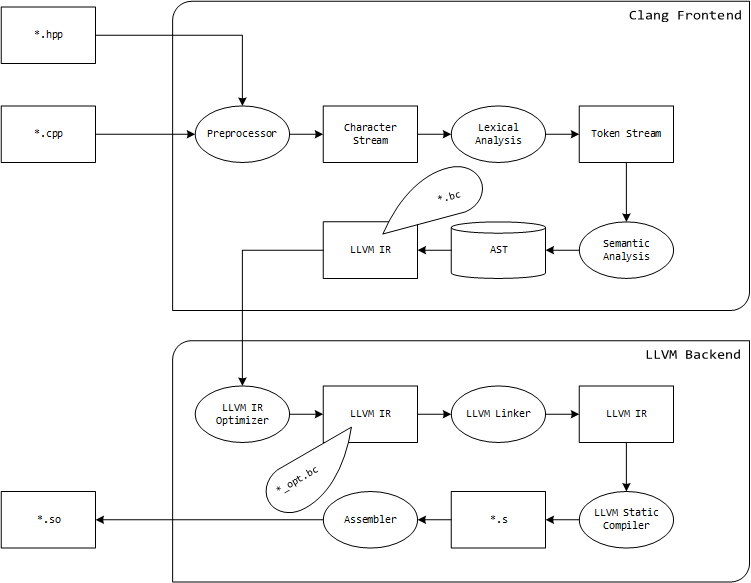
\includegraphics[width=0.8\textwidth]{images/LLVM.png}
\end{figure}

\begin{enumerate}
    \item \textbf{Preprocessing:} Evaluates all preprocessor directives (string
    concatenation) in memory and creates a character stream for further processing.
    \item \textbf{Lexical Analysis:} Reads and analyzes the incoming character
    stream by dividing it into tokens, each of which corresponds to a certain symbol
    in the source language (for example keywords, variable names or numbers). 
    \item \textbf{Syntax Analysis:} Parses the token stream and produces an abstract
    syntax tree that reflects the structure of the program.
    \item \textbf{Type Checking:} Examines the abstract syntax tree and determines
    if the program violates the semantic rules of the language (for example when
    a variable is used but not declared, or when a Boolean value is treated like
    a function pointer).
    \item \textbf{Intermediate Code Generation:} Translates the program into a
    machine-independent language (for example LLVM IR). This is also where most
    of the code optimization takes place.
    \item \textbf{Machine Code Generation:} Translates LLVM IR to assembly language
    for a specific machine architecture.
    \item \textbf{Assembly and Linking:} The assembler creates an object file,
    i.e., determines a binary representation and addresses of variables, function
    names, and so on \autocite{mogensen2010}.
\end{enumerate}

When the source language is also the implementation language\footnote{The language
the compiler itself is written in.} and the source text to be compiled is actually
a new version of the compiler itself, the process is called bootstrapping\footnote{This
is an advanced topic that is outside the scope of this document. For more information
see also: \url{https://en.wikipedia.org/wiki/Compiler-compiler}.} \autocite{grune2012}.
In case of C or C++ it is more appropriate to say that an ahead-of-time compilation
(AOT) takes place when the IR is lifted down to native machine code before the program
is executed. This is different from using a just-in-time (JIT) compiler in an alternative
implementation of Python.

LLVM IR is a RISC-like set of instructions that is capable of expressing statically
typed high-level language constructs with an infinite amount of function local
registers and is available in form of two file formats, bitcode (\texttt{.bc}) and
human-readable code (\texttt{.ll}). This intermediate code generation makes it
possible to link files that were originally written in different high-level languages,
such as C, C++, Go, Rust or Swift and enables efficient code optimization. At its
core, an IR module consists of three things: target information, global symbols
and miscellaneous other data.

\begin{figure}[ht]
    \centering
    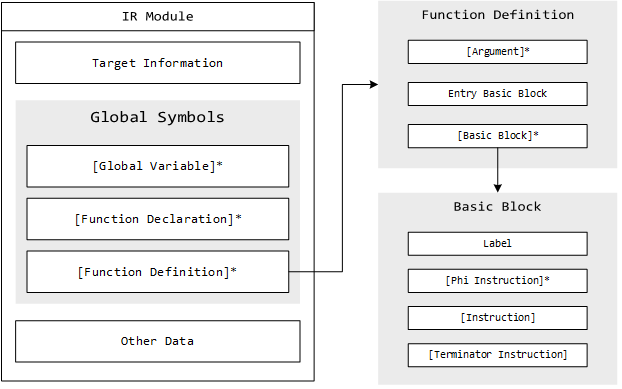
\includegraphics[width=0.7\textwidth]{images/LLVMIR.png}
\end{figure}

The target information starts with a pair of strings describing the target. For
example, the target layout string describes:

\begin{itemize}
    \item The endianness
    \item ELF mangling
    \item ABI alignment of i64
    \item Native integer widths
\end{itemize}

Moreover, the target triple string contains information about 

\begin{itemize}
    \item The architecture
    \item Vendor
    \item System
    \item ABI
\end{itemize}

A function definition, for instance, contains zero or more arguments, an entry
block as well as zero or more basic blocks. A basic block contains a label, zero
or more phi instructions, and zero or more instructions followed by the terminator
instruction. One of the main characteristics of a basic block is the control sequence:
it is written in SSA-form (Static Single Assignment), meaning that each register
is assigned exactly once which greatly simplifies control flow analysis. Phi
instructions return one value from a set of incoming values based on the control
flow path taken during execution to reach the phi instruction where each value is
associated with a predecessor basic block. An instruction performs arithmetic
operations or accesses the memory but doesn't alter the flow of the program. The
terminator instruction determines the control flow transfer once the basic block
finishes its execution. 
